\documentclass[aspectratio=43,9pt]{beamer}
%
\usepackage{graphicx,tikz}
%
\usetheme{Boadilla}
%
\graphicspath{{./figures/nt7/}}
%
\let\Tiny=\tiny%			% to avoid warnings about font size
%\usepackage{lmodern}%		% alternative method to avoid these warnings
%
\catcode`~=11 % make LaTeX treat tilde (~) like a normal character
\newcommand{\urltilde}{\hbox{~}}
\catcode`~=13 % revert back to treating tilde (~) as an active character
%
% misc commands
\newcommand{\bm}[1]{\mathbf{#1}}
\newcommand{\bs}[1]{\boldsymbol{#1}}
\newenvironment{myitemize}[1]{\vspace{#1}\begin{itemize}\setlength\itemsep{#1}}{\end{itemize}}
%
% pgf markers
\usepgflibrary{plotmarks}
%
\setbeamertemplate{footline}
{
  \leavevmode%
  \hbox{%
  \begin{beamercolorbox}[wd=.8\paperwidth,ht=2.25ex,dp=1ex,left]{author in head/foot}%
    \usebeamerfont{author in head/foot}\hspace*{4em}\inserttitle
  \end{beamercolorbox}%
  \begin{beamercolorbox}[wd=.2\paperwidth,ht=2.25ex,dp=1ex,right]{author in head/foot}%
    \usebeamerfont{author in head/foot}\insertframenumber{} / \inserttotalframenumber\hspace*{1ex}
  \end{beamercolorbox}}%
  \vskip0pt%
}
%
\setbeamertemplate{navigation symbols}{}
%
\setbeamertemplate{frametitle}
{%
	\begin{minipage}{.9\paperwidth}
		\vspace*{1ex}%
		\flushright%
		%\bfseries
		\LARGE%
		\insertframetitle%
	\end{minipage}%
}
%
\setbeamertemplate{title page}{
	\begin{center}
		\vspace*{2ex}
		\usebeamercolor[fg]{frametitle}{%
			\Large%
			Numerical Techniques 2025--2026\\[2ex]
			%
			\LARGE%
			\inserttitle
		}\\[6ex]
		\usebeamercolor[fg]{normal text}{%
			Daan Degrauwe\\[1ex]
			\texttt{daan.degrauwe@meteo.be}\\[4ex]
			Postgraduate Studies in Weather and Climate Modeling\\[1ex]
			Ghent University
		}
	\end{center}
}
%
\newcommand{\ft}[2]{{\textstyle\frac{#1}{#2}}}
%
% increase space around equations
\makeatletter
\g@addto@macro\normalsize{%
	\setlength{\abovedisplayskip}{3ex}%
	\setlength{\belowdisplayskip}{3ex}%
	\setlength{\abovedisplayshortskip}{3ex}%
	\setlength{\belowdisplayshortskip}{3ex}%
}%
\makeatother
%

%
\title{7. Parallel computing and implications in NWP}%
%
%%%%%%%%%%%%%%%%%%%%%%%%%%%%%%%%%%%%%%%%%%%%%%%%%%%%%%%%%%%%%%%%%%%%%%
%
\begin{document}
%
%%%%%%%%%%%%%%%%%%%%%%%%%%%%%%%%%%%%%%%%%%%%%%%%%%%%%%%%%%%%%%%%%%%%%%%%%%%%%%%%%%%%%%%%%%%%%%%%%%%%
%
\begin{frame}[plain]
	\titlepage
\end{frame}
%
%%%%%%%%%%%%%%%%%%%%%%%%%%%%%%%%%%%%%%%%%%%%%%%%%%%%%%%%%%%%%%%%%%%%%%
%
\begin{frame}
	%
	\frametitle{Content}
	%
	\begin{myitemize}{4ex}
		\item General aspects of parallel computing:
			%
			\begin{myitemize}{2ex}
				\item Introduction
				\item Amdahl's law
				\item Shared  and distributed memory
			\end{myitemize}
			%
		\item NWP-specificities
			\begin{myitemize}{2ex}
				\item Design of an NWP model; `physics' and `dynamics'
				\item Parallelization in physics
				\item Parallelization in dynamics
				\item The future?
			\end{myitemize}
			%
	\end{myitemize}
	%
\end{frame}
%
%%%%%%%%%%%%%%%%%%%%%%%%%%%%%%%%%%%%%%%%%%%%%%%%%%%%%%%%%%%%%%%%%%%%%%
%
\begin{frame}
	%
	\frametitle{Introduction}
	%
	\begin{myitemize}{2ex}
		\item We want to run forecasts as quickly as possible\ldots
			%
		\item Until $\sim$ 2003, performance was increased by making processors \emph{faster}
			\begin{center}
				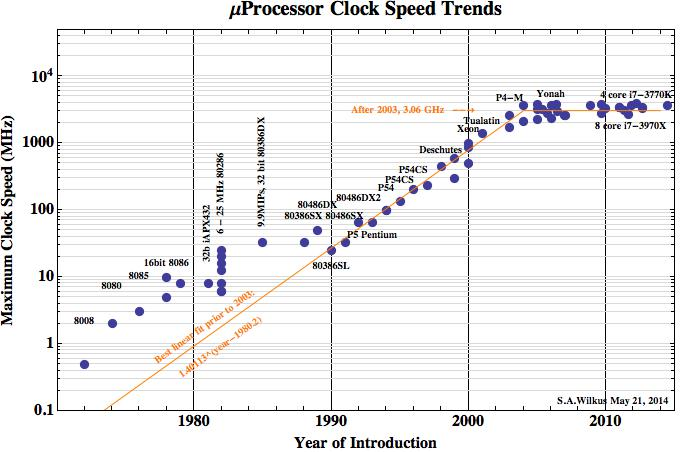
\includegraphics[width=6cm]{clocktrends}
			\end{center}
			%
		\item It seems that increasing the clock frequency above 3GHz isn't beneficial (power consumption!)
			%
	\end{myitemize}
	%
\end{frame}
%
%%%%%%%%%%%%%%%%%%%%%%%%%%%%%%%%%%%%%%%%%%%%%%%%%%%%%%%%%%%%%%%%%%%%%%
%
\begin{frame}
	%
	\frametitle{Introduction}
	%
	\begin{myitemize}{2ex}
		\item So we'll just use \emph{more} processors instead of faster ones.
		\item For example: ECMWF's Cray machine
			%
			\begin{center}\vspace*{2ex}
				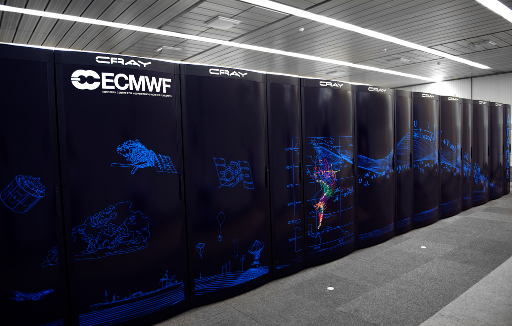
\includegraphics[width=6cm]{cray}
			\end{center}\vspace*{2ex}
			%
			with 260'000 cores, or RMI's machine with 2688 cores
	\end{myitemize}
\end{frame}
%
%%%%%%%%%%%%%%%%%%%%%%%%%%%%%%%%%%%%%%%%%%%%%%%%%%%%%%%%%%%%%%%%%%%%%%
%
\begin{frame}
	%
	\frametitle{Unparallelizable problems}
	%
	\begin{myitemize}{2ex}
		\item Not everything goes faster when you use multiple processors!
			%
		\item For instance: Newton-Raphson iterative method to find a root of a function $f(x)$:
			%
			\begin{equation*}
				x_{i+1}=x_i-\frac{f(x_i)}{f'(x_i)}
			\end{equation*}
			%
			$x_i$ is required for the calculation of $x_{i+1}$, so the different iterations cannot be performed by different processors.
			%
		\item IO (Input/Output), i.e. writing and reading to disk is another example.
			%
	\end{myitemize}
	%
\end{frame}
%
%%%%%%%%%%%%%%%%%%%%%%%%%%%%%%%%%%%%%%%%%%%%%%%%%%%%%%%%%%%%%%%%%%%%%%
%
\begin{frame}
	%
	\frametitle{Amdahl's law}
	%
	\begin{myitemize}{2ex}
		\item Consider a program consisting of two parts
			%
			\begin{enumerate}\vspace*{2ex}
				\item a part that cannot be parallelized: the \emph{serial} part $S$. This part is responsible for a fraction $\sigma$ of the total time $T_1$ on a single processor.\vspace*{2ex}
				\item a parallelizable part $P$. This parts is responsible for a fraction $1-\sigma$ of the total time on a single processor.
			\end{enumerate}
			%
		\item Then in a parallel environment with $n$ processors, the total time will be
			%
			\begin{equation*}
				T_n=\sigma T_1 + \frac{1-\sigma}{n} T_1
			\end{equation*}
			%
			So the speed-up is
			%
			\begin{equation*}
				\frac{T_1}{T_n}=\frac{1}{\sigma + \frac{1-\sigma}{n}}
			\end{equation*}
			%
	\end{myitemize}
	%
\end{frame}
%
%%%%%%%%%%%%%%%%%%%%%%%%%%%%%%%%%%%%%%%%%%%%%%%%%%%%%%%%%%%%%%%%%%%%%%
%
\begin{frame}
	%
	\frametitle{Amdahl's law}
	%
	\begin{myitemize}{2ex}
		\item Speedup as a function of the number of processors:
			%
			\begin{center}
				%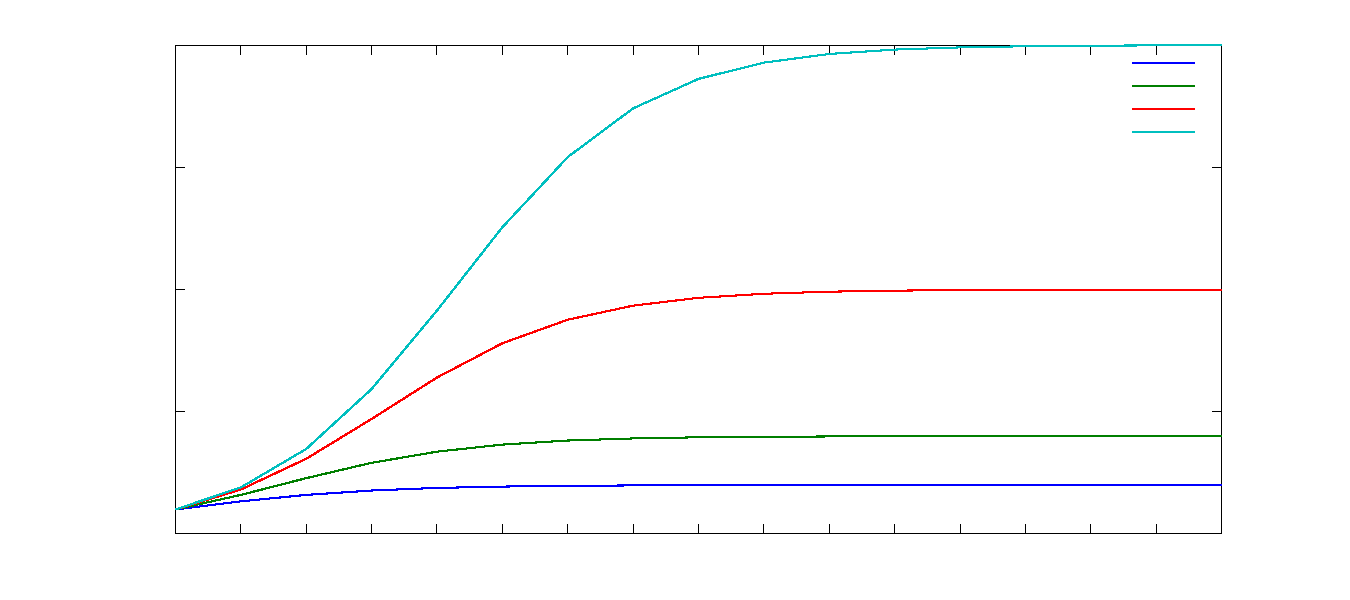
\includegraphics[width=7cm]{amdahl}
				\scalebox{.5}{% GNUPLOT: LaTeX picture with Postscript
\begingroup
  \makeatletter
  \providecommand\color[2][]{%
    \GenericError{(gnuplot) \space\space\space\@spaces}{%
      Package color not loaded in conjunction with
      terminal option `colourtext'%
    }{See the gnuplot documentation for explanation.%
    }{Either use 'blacktext' in gnuplot or load the package
      color.sty in LaTeX.}%
    \renewcommand\color[2][]{}%
  }%
  \providecommand\includegraphics[2][]{%
    \GenericError{(gnuplot) \space\space\space\@spaces}{%
      Package graphicx or graphics not loaded%
    }{See the gnuplot documentation for explanation.%
    }{The gnuplot epslatex terminal needs graphicx.sty or graphics.sty.}%
    \renewcommand\includegraphics[2][]{}%
  }%
  \providecommand\rotatebox[2]{#2}%
  \@ifundefined{ifGPcolor}{%
    \newif\ifGPcolor
    \GPcolortrue
  }{}%
  \@ifundefined{ifGPblacktext}{%
    \newif\ifGPblacktext
    \GPblacktexttrue
  }{}%
  % define a \g@addto@macro without @ in the name:
  \let\gplgaddtomacro\g@addto@macro
  % define empty templates for all commands taking text:
  \gdef\gplbacktext{}%
  \gdef\gplfronttext{}%
  \makeatother
  \ifGPblacktext
    % no textcolor at all
    \def\colorrgb#1{}%
    \def\colorgray#1{}%
  \else
    % gray or color?
    \ifGPcolor
      \def\colorrgb#1{\color[rgb]{#1}}%
      \def\colorgray#1{\color[gray]{#1}}%
      \expandafter\def\csname LTw\endcsname{\color{white}}%
      \expandafter\def\csname LTb\endcsname{\color{black}}%
      \expandafter\def\csname LTa\endcsname{\color{black}}%
      \expandafter\def\csname LT0\endcsname{\color[rgb]{1,0,0}}%
      \expandafter\def\csname LT1\endcsname{\color[rgb]{0,1,0}}%
      \expandafter\def\csname LT2\endcsname{\color[rgb]{0,0,1}}%
      \expandafter\def\csname LT3\endcsname{\color[rgb]{1,0,1}}%
      \expandafter\def\csname LT4\endcsname{\color[rgb]{0,1,1}}%
      \expandafter\def\csname LT5\endcsname{\color[rgb]{1,1,0}}%
      \expandafter\def\csname LT6\endcsname{\color[rgb]{0,0,0}}%
      \expandafter\def\csname LT7\endcsname{\color[rgb]{1,0.3,0}}%
      \expandafter\def\csname LT8\endcsname{\color[rgb]{0.5,0.5,0.5}}%
    \else
      % gray
      \def\colorrgb#1{\color{black}}%
      \def\colorgray#1{\color[gray]{#1}}%
      \expandafter\def\csname LTw\endcsname{\color{white}}%
      \expandafter\def\csname LTb\endcsname{\color{black}}%
      \expandafter\def\csname LTa\endcsname{\color{black}}%
      \expandafter\def\csname LT0\endcsname{\color{black}}%
      \expandafter\def\csname LT1\endcsname{\color{black}}%
      \expandafter\def\csname LT2\endcsname{\color{black}}%
      \expandafter\def\csname LT3\endcsname{\color{black}}%
      \expandafter\def\csname LT4\endcsname{\color{black}}%
      \expandafter\def\csname LT5\endcsname{\color{black}}%
      \expandafter\def\csname LT6\endcsname{\color{black}}%
      \expandafter\def\csname LT7\endcsname{\color{black}}%
      \expandafter\def\csname LT8\endcsname{\color{black}}%
    \fi
  \fi
  \setlength{\unitlength}{0.0500bp}%
  \begin{picture}(12960.00,5760.00)%
    \gplgaddtomacro\gplbacktext{%
      \colorrgb{0.00,0.00,0.00}%
      \put(1552,634){\makebox(0,0)[r]{\strut{}0}}%
      \colorrgb{0.00,0.00,0.00}%
      \put(1552,1807){\makebox(0,0)[r]{\strut{}5}}%
      \colorrgb{0.00,0.00,0.00}%
      \put(1552,2981){\makebox(0,0)[r]{\strut{}10}}%
      \colorrgb{0.00,0.00,0.00}%
      \put(1552,4154){\makebox(0,0)[r]{\strut{}15}}%
      \colorrgb{0.00,0.00,0.00}%
      \put(1552,5327){\makebox(0,0)[r]{\strut{}20}}%
      \colorrgb{0.00,0.00,0.00}%
      \put(1684,414){\makebox(0,0){\strut{}    1}}%
      \colorrgb{0.00,0.00,0.00}%
      \put(2312,414){\makebox(0,0){\strut{}    2}}%
      \colorrgb{0.00,0.00,0.00}%
      \put(2940,414){\makebox(0,0){\strut{}    4}}%
      \colorrgb{0.00,0.00,0.00}%
      \put(3567,414){\makebox(0,0){\strut{}    8}}%
      \colorrgb{0.00,0.00,0.00}%
      \put(4195,414){\makebox(0,0){\strut{}   16}}%
      \colorrgb{0.00,0.00,0.00}%
      \put(4823,414){\makebox(0,0){\strut{}   32}}%
      \colorrgb{0.00,0.00,0.00}%
      \put(5451,414){\makebox(0,0){\strut{}   64}}%
      \colorrgb{0.00,0.00,0.00}%
      \put(6078,414){\makebox(0,0){\strut{}  128}}%
      \colorrgb{0.00,0.00,0.00}%
      \put(6706,414){\makebox(0,0){\strut{}  256}}%
      \colorrgb{0.00,0.00,0.00}%
      \put(7334,414){\makebox(0,0){\strut{}  512}}%
      \colorrgb{0.00,0.00,0.00}%
      \put(7962,414){\makebox(0,0){\strut{} 1024}}%
      \colorrgb{0.00,0.00,0.00}%
      \put(8589,414){\makebox(0,0){\strut{} 2048}}%
      \colorrgb{0.00,0.00,0.00}%
      \put(9217,414){\makebox(0,0){\strut{} 4096}}%
      \colorrgb{0.00,0.00,0.00}%
      \put(9845,414){\makebox(0,0){\strut{} 8192}}%
      \colorrgb{0.00,0.00,0.00}%
      \put(10473,414){\makebox(0,0){\strut{}16384}}%
      \colorrgb{0.00,0.00,0.00}%
      \put(11100,414){\makebox(0,0){\strut{}32768}}%
      \colorrgb{0.00,0.00,0.00}%
      \put(11728,414){\makebox(0,0){\strut{}65536}}%
      \colorrgb{0.00,0.00,0.00}%
      \put(1046,2980){\rotatebox{90}{\makebox(0,0){\strut{}Speedup}}}%
      \colorrgb{0.00,0.00,0.00}%
      \put(6706,84){\makebox(0,0){\strut{}Number of processors}}%
    }%
    \gplgaddtomacro\gplfronttext{%
      \csname LTb\endcsname%
      \put(10741,5154){\makebox(0,0)[r]{\strut{}50\%}}%
      \csname LTb\endcsname%
      \put(10741,4934){\makebox(0,0)[r]{\strut{}75\%}}%
      \csname LTb\endcsname%
      \put(10741,4714){\makebox(0,0)[r]{\strut{}90\%}}%
      \csname LTb\endcsname%
      \put(10741,4494){\makebox(0,0)[r]{\strut{}95\%}}%
    }%
    \gplbacktext
    \put(0,0){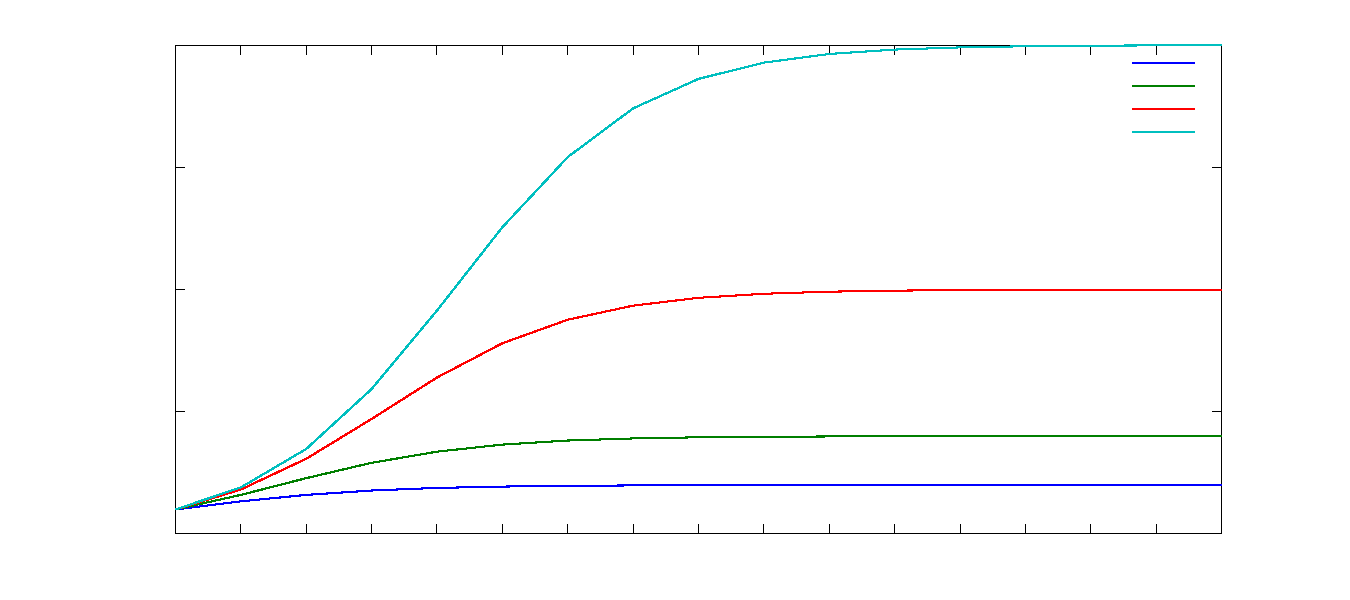
\includegraphics{amdahl}}%
    \gplfronttext
  \end{picture}%
\endgroup
}
			\end{center}
			%
		\item So there's a limit to the speed-up that can be achieved by parallelizing! We call this the \emph{scalability} of a program.
			%
	\pause
		\item But in fact, this isn't even the biggest challenge in NWP/Climate on high-performance systems.
			%
	\end{myitemize}
	%
\end{frame}
%
%%%%%%%%%%%%%%%%%%%%%%%%%%%%%%%%%%%%%%%%%%%%%%%%%%%%%%%%%%%%%%%%%%%%%%
%
\begin{frame}
	%
	\frametitle{Shared and distributed memory}
	%
	\begin{myitemize}{2ex}
		\item Memory is the part of a computer where data are stored temporarily, right before/after the numerical operations.
			%
		\item The most convenient setup is where all processors can access some central memory, and divide the work 
			%
			\begin{center}
				\begin{tikzpicture}
					\draw (3,-1) node {
\includegraphics[width=3cm]{pie_full}};
					\draw (0,0) node {
\includegraphics[width=2.13cm,height=2.37cm]{monster}};
					\draw (4,0) node {
\includegraphics[width=-2.13cm,height=2.37cm]{monster}};
					\draw (6,0);
				\end{tikzpicture}
			\end{center}
			%
		\item We call this a \emph{shared} memory environment
			%
		\item The standard for shared-memory parallelization is \emph{OpenMP}
			%
	\end{myitemize}
	%
\end{frame}
%
%%%%%%%%%%%%%%%%%%%%%%%%%%%%%%%%%%%%%%%%%%%%%%%%%%%%%%%%%%%%%%%%%%%%%%
%
\begin{frame}
	%
	\frametitle{Shared and distributed memory}
	%
	\begin{myitemize}{2ex}
		\item Due to hardware constraints, shared memory becomes unfeasible for large systems
			%
		\item In such systems, every processor is attributed his own piece of memory, and other processors cannot access it.
			%
			\begin{center}
				\begin{tikzpicture}
					\draw (1,-1) node {
\includegraphics[width=1.5cm]{pie_piece}};
					\draw (5,-1) node {
\includegraphics[width=1.5cm]{pie_piece}};
					\draw (-1,0) node {
\includegraphics[width=2.13cm,height=2.37cm]{monster}};
					\draw (5,0) node {
\includegraphics[width=-2.13cm,height=2.37cm]{monster}};
					\draw[line width=2pt] (3,-2) -- (3,2);
					\draw (7,0);
				\end{tikzpicture}
			\end{center}
			%
		\item We call this a \emph{distributed} memory environment
			%
	\end{myitemize}
	%
\end{frame}
%
%%%%%%%%%%%%%%%%%%%%%%%%%%%%%%%%%%%%%%%%%%%%%%%%%%%%%%%%%%%%%%%%%%%%%%
%
\begin{frame}
	%
	\frametitle{Shared and distributed memory}
	%
	\begin{myitemize}{2ex}
		\item In a distributed memory environment, communication between processors has to be coded explicitly through \emph{messages}.
			%
		\item For instance:
			%
			\begin{enumerate}\vspace*{1ex}\setlength\itemsep{1ex}
				\item Processor 1 reads some data from a file;
				\item Processor 1 \emph{sends} (pieces of) the data to the other processors $2-n$;
				\item Processors $1-n$ process their piece of data;
				\item Processors $2-n$ \emph{send} their result back to processor 1;
				\item Processor 1 writes the results to a file.
			\end{enumerate}
			%
		\item The standard for distributed memory parallelization is \emph{MPI} (Message Passing Interface).
			%
		\item The cost of communications (slowly) \emph{increases} with the number of processors:
			\begin{itemize}
				\item number of messages increases
				\item message sizes decrease
				\item processors are further apart
			\end{itemize}
	\end{myitemize}
	%
\end{frame}
%
%%%%%%%%%%%%%%%%%%%%%%%%%%%%%%%%%%%%%%%%%%%%%%%%%%%%%%%%%%%%%%%%%%%%%%
%
\begin{frame}
	%
	\frametitle{Shared and distributed memory}
	%
	\begin{myitemize}{2ex}
		%
		\item Multicore processors allow for hybrid systems:
			\begin{myitemize}{1ex}
				\item \emph{within} a processor (i.e. between different cores of the same processor), memory is shared, and OpenMP is used for parallelization
				\item \emph{between} processors, memory is distributed, and MPI is used for communication
			\end{myitemize}
			%
			\begin{center}\vspace*{1ex}\hspace*{-1cm}
				\scalebox{.9}{%
					\begin{tikzpicture}[>=latex]
						\draw (1,-1) node {
\includegraphics[width=1.5cm]{pie_piece}};
						\draw (5,-1) node {
\includegraphics[width=1.5cm]{pie_piece}};
						\draw (-1,0) node {
\includegraphics[width=2.13cm,height=2.37cm]{monster3}};
						\draw (4.87,0) node {
\includegraphics[width=-2.13cm,height=2.37cm]{monster3}};
						\draw (-3,1.5) node (cc) {core 1}; \draw[->] (cc)  -- (-2,.8);
						\draw  (-1,2) node (cc) {core 2}; \draw[->] (cc) -- (-1,1);
						\draw  (1,1.5) node (cc) {core 3}; \draw[->] (cc) -- (0,.8);
						\draw (-1,-2) node {\large Processor 1};
						\draw  (5,1.5) node (cc) {core 1}; \draw[->] (cc) -- (6,.8);
						\draw  (7,2) node (cc) {core 2}; \draw[->] (cc) -- (7,1);
						\draw  (9,1.5) node (cc) {core 3}; \draw[->] (cc) -- (8,.8);
						\draw (7,-2) node {\large Processor 2};
						\draw[line width=2pt] (3,-2) -- (3,2);
					\end{tikzpicture}
				}
			\end{center}
			%
	\end{myitemize}
	%
\end{frame}
%
%%%%%%%%%%%%%%%%%%%%%%%%%%%%%%%%%%%%%%%%%%%%%%%%%%%%%%%%%%%%%%%%%%%%%%
%
\begin{frame}
	%
	\frametitle{Design of an NWP model}
	%
	\begin{myitemize}{3ex}
		\item Almost all NWP models consist of a `dynamical part' and a `physical part'.
			%
		\item Dynamics (3D) are conservation of mass, energy, momentum; perfect gas law.
			%
		\item The dynamics of the ALADIN/ARPEGE/IFS model are
			%
			\begin{myitemize}{1ex}
				\item spectral
				\item semi-implicit
				\item semi-Lagrangian
				\item for LAM: Davies coupling to global model (ARPEGE/IFS)
				\item terrain-following hybrid pressure coordinate
				\item hydrostatic and nonhydrostatic
			\end{myitemize}
			%
	\end{myitemize}
	%
\end{frame}
%
%%%%%%%%%%%%%%%%%%%%%%%%%%%%%%%%%%%%%%%%%%%%%%%%%%%%%%%%%%%%%%%%%%%%%%
%
\begin{frame}
	%
	\frametitle{Design of an NWP model}
	%
	\begin{myitemize}{2ex}
		\item The physics part models the \emph{unresolved} or \emph{subscale} phenomena: turbulence, radiation, diffusion, clouds, precipitation, surface, \ldots
			%
			\begin{center}
				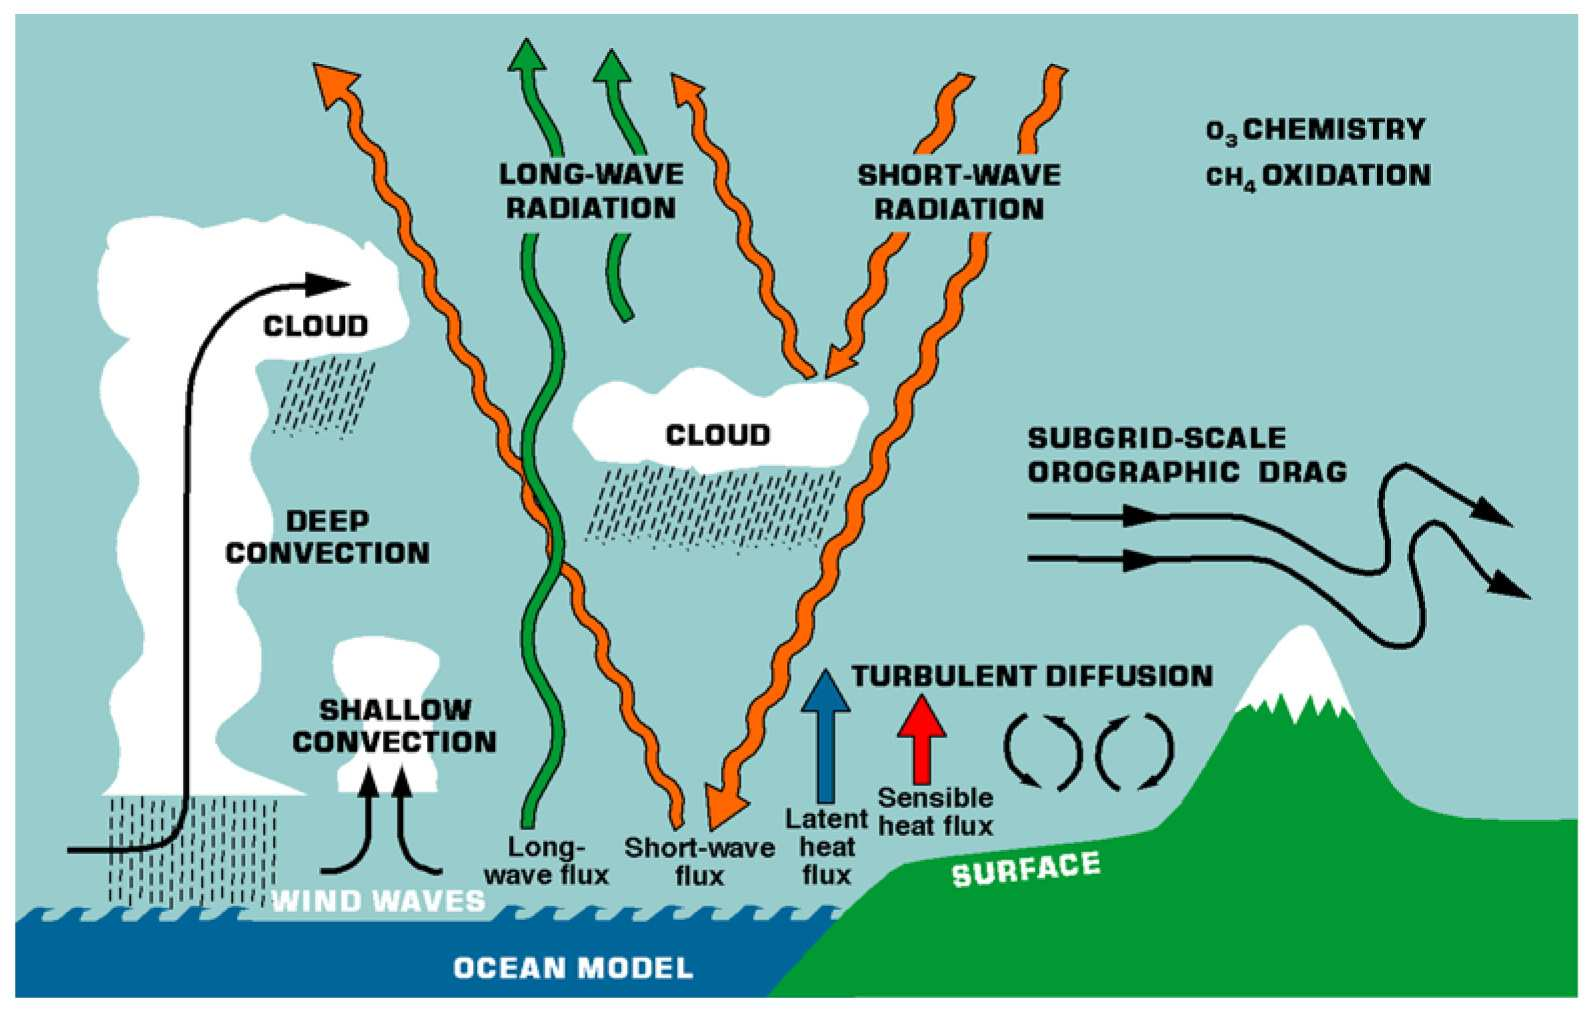
\includegraphics[width=.7\textwidth]{physics}
			\end{center}
			%
	\end{myitemize}
	%
\end{frame}
%
%%%%%%%%%%%%%%%%%%%%%%%%%%%%%%%%%%%%%%%%%%%%%%%%%%%%%%%%%%%%%%%%%%%%%%
%
\begin{frame}
	%
	\frametitle{Design of an NWP model}
	%
	A single timestep of the spectral ALADIN model looks like:
	%
	\begin{enumerate}\vspace*{2ex}\setlength\itemsep{2ex}
		\item calculate derivatives in spectral space
		\item apply explicit part of \emph{dynamics}
		\item Fourier transform to gridpoint space
		\item semi-Lagrangian interpolations and nonlinear dynamical terms
		\item calculate \emph{physics} contributions to energy and momentum equations
		\item apply \emph{boundary conditions}
		\item Fourier transform to spectral space
		\item solve implicit operator (\emph{dynamics})
	\end{enumerate}	
	%
\end{frame}
%
%%%%%%%%%%%%%%%%%%%%%%%%%%%%%%%%%%%%%%%%%%%%%%%%%%%%%%%%%%%%%%%%%%%%%%
%
\begin{frame}
	%
	\frametitle{Parallelization in the physics}
	%
	\begin{myitemize}{2ex}
		\item Most physics phenomena act mainly in the vertical (e.g. precipitation, stability, \ldots)
			%
		\item The physics are computed in vertical columns
			%
			\begin{center}
				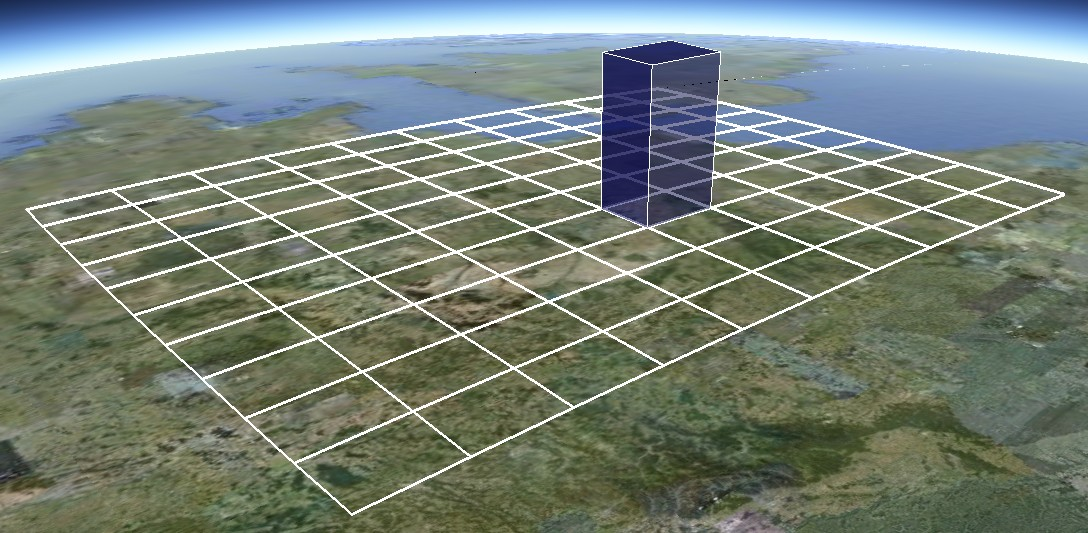
\includegraphics[width=8cm]{column}
			\end{center}
			%
		\item There's no interaction (so no communication!) between the columns
			%
		\item So the physics scale very well (quasi-perfectly!).
			%
		\item (the column-approach may become problematic for very high resolutions)
			%
	\end{myitemize}
	%
\end{frame}
%
%%%%%%%%%%%%%%%%%%%%%%%%%%%%%%%%%%%%%%%%%%%%%%%%%%%%%%%%%%%%%%%%%%%%%%
%
\begin{frame}
	%
	\frametitle{Dynamics parallelization: spectral dynamics}
	%
	\begin{myitemize}{2ex}
		\item The spectral dynamics are parallelized by distributing the wavelengths over the processors.
			%
		\item The Fourier transforms are quite communication-intensive!
			%
			\begin{align*}
				f(x_j)		&=\sum_{k=-N/2}^{k=N/2} \alpha_k \exp(i k x_j)	\\
				\alpha_k	&=\frac{1}{N}\sum_{j=1}^N f(x_j) \exp(- i k x_j)
			\end{align*}
			%
			So a wave amplitude depends on \emph{all} gridpoints, and vice versa; a gridpoint value is the combination of \emph{all} composing waves.
			%
		\item We say that the Fourier transform is \emph{not local} (as opposed to finite differences)
			%
		\item \textbf{Note}: this nonlocality is also the key to the high accuracy of spectral methods.
			%
	\end{myitemize}
	%
\end{frame}
%
%%%%%%%%%%%%%%%%%%%%%%%%%%%%%%%%%%%%%%%%%%%%%%%%%%%%%%%%%%%%%%%%%%%%%%
%
\begin{frame}
	%
	\frametitle{Dynamics parallelization: semi-Lagrangian advection}
	%
	\begin{myitemize}{2ex}
		\item Semi-Lagrangian calculations require interaction with nearby processors: the trajectory departure points may well belong to another processor.
			\begin{center}
				\begin{tikzpicture}[>=latex]
					\draw[use as bounding box] (0,0) node {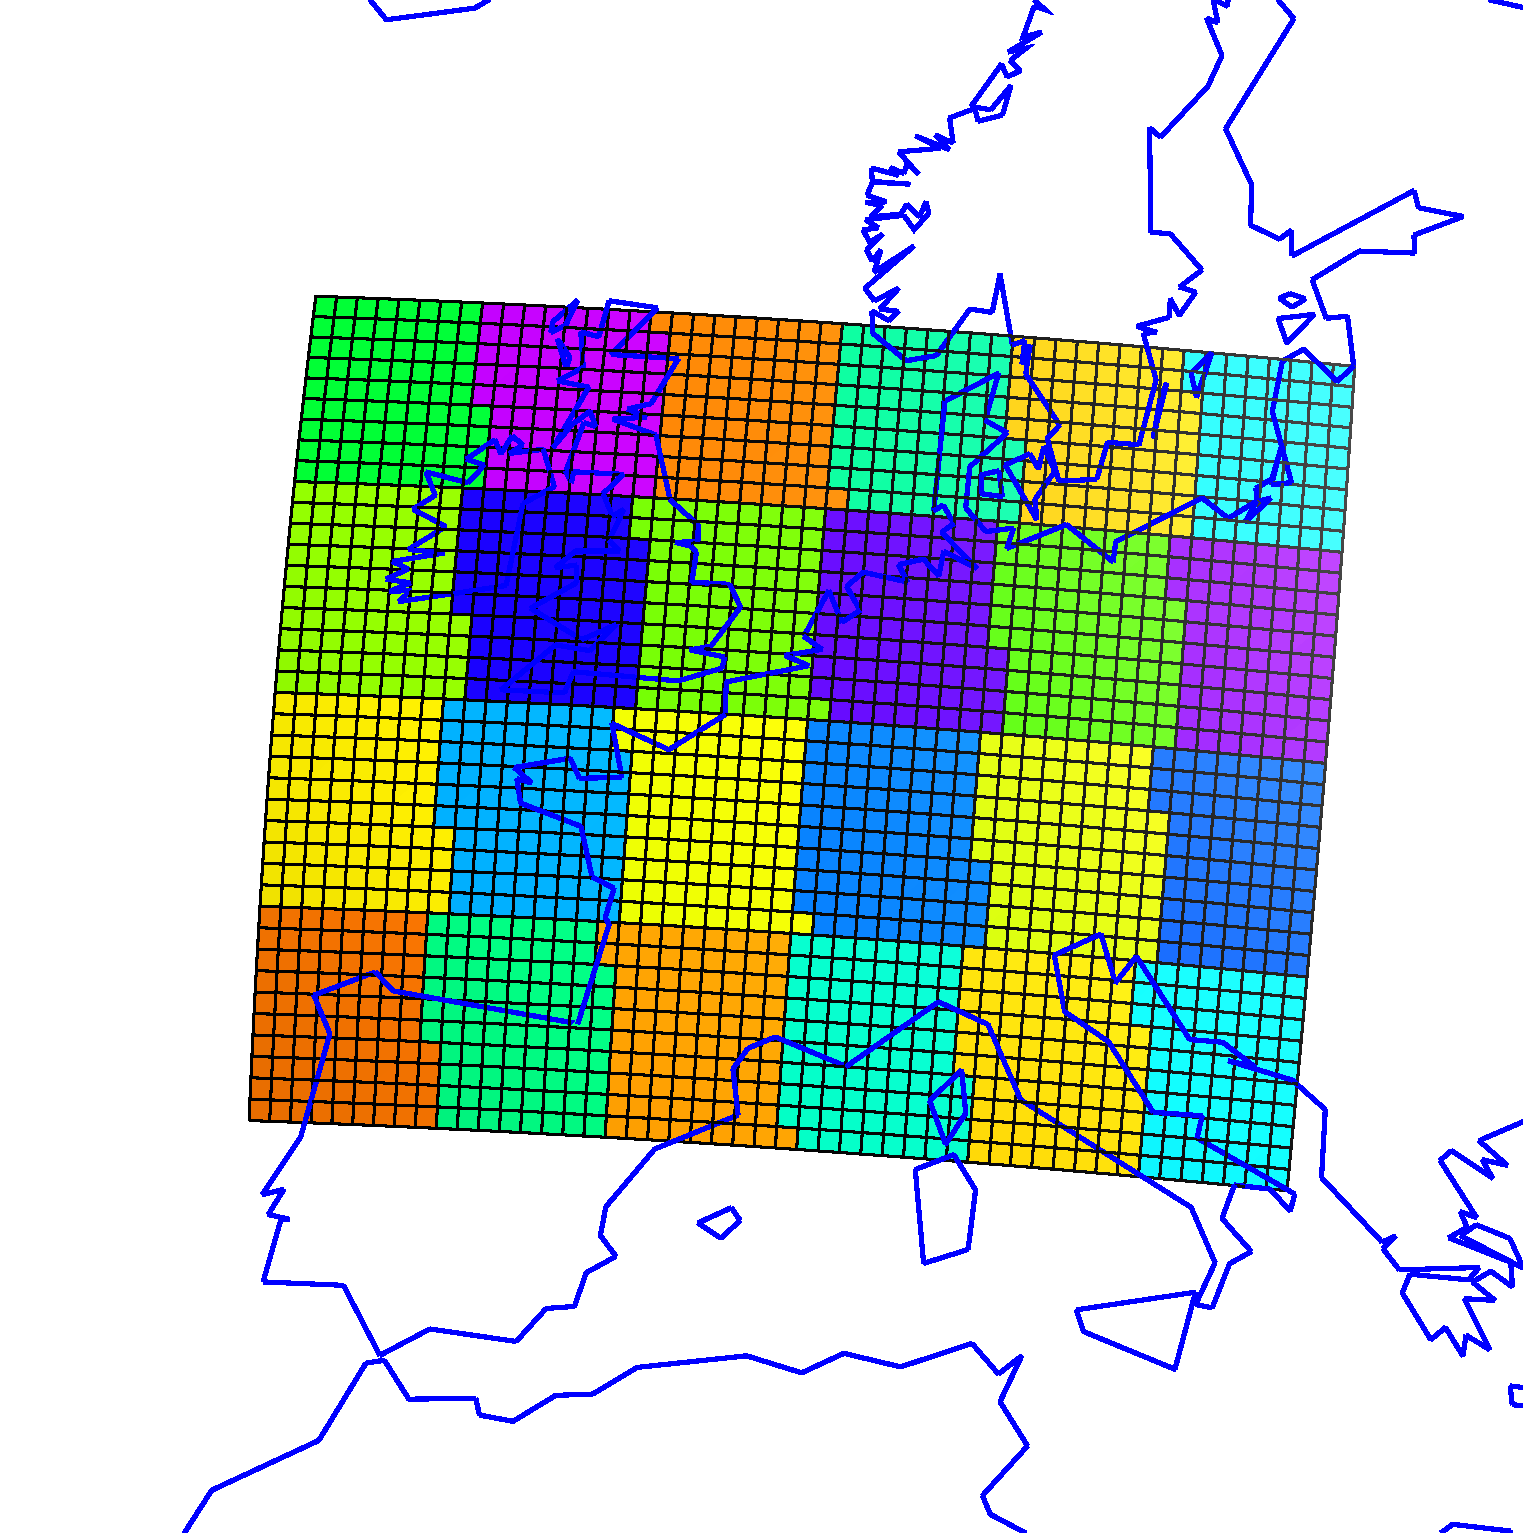
\includegraphics[width=.4\textwidth]{LAM1}}; 
					\draw (0,0) node {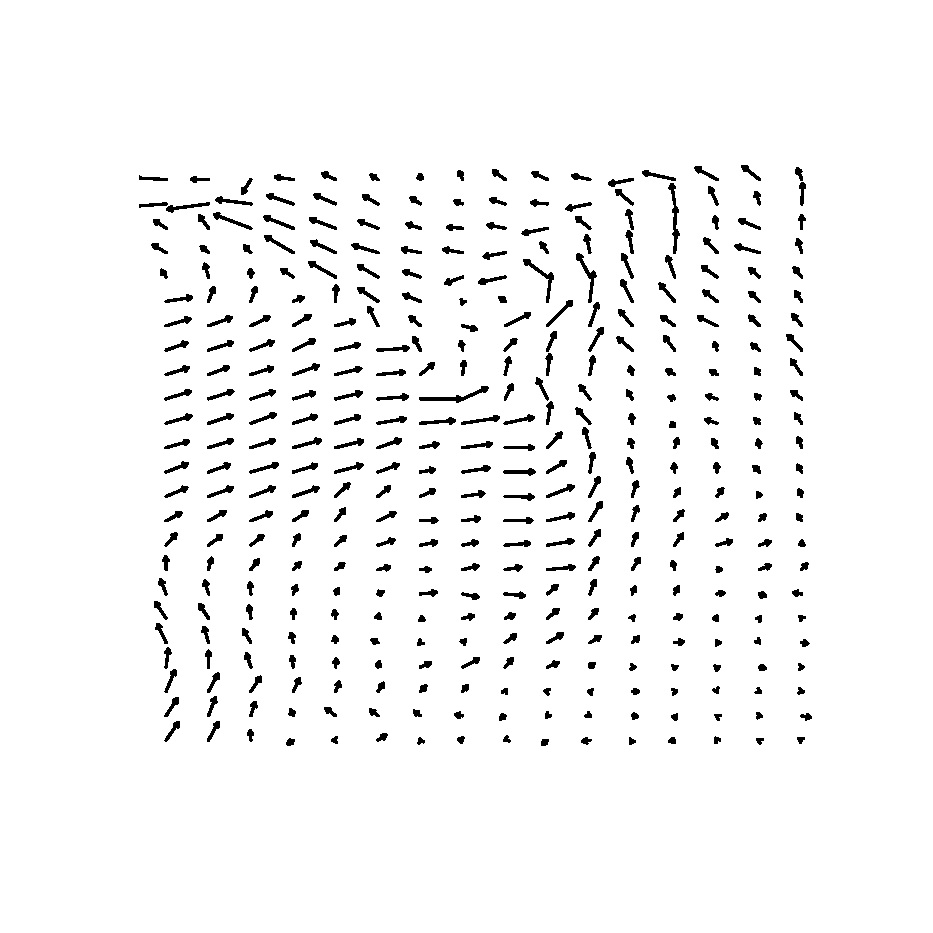
\includegraphics[width=.6\textwidth]{wind}}; 
				\end{tikzpicture}%
			\end{center}
	\end{myitemize}
	%
\end{frame}
%
%%%%%%%%%%%%%%%%%%%%%%%%%%%%%%%%%%%%%%%%%%%%%%%%%%%%%%%%%%%%%%%%%%%%%%
%
\begin{frame}
	%
	\frametitle{Dynamics parallelization: implicit timestepping}
	%
	\begin{myitemize}{2ex}
		\item Implicit timestepping is also not local, even when using finite differences.
		\item For example, the trapezium scheme for the advection equation
		%
			\begin{equation*}
				\frac{\phi_{j}^{n+1}-\phi_{j}^n}{\Delta t}+\frac{c}{2}\left(\frac{\phi^{n+1}_{j+1}-\phi^{n+1}_{j-1}}{2\Delta x}+\frac{\phi^{n}_{j+1}-\phi^{n}_{j-1}}{2\Delta x}\right)=0
			\end{equation*}
			%
			leads to a tridiagonal linear system that needs to be solved every timestep:
			%
			\begin{equation*}
				\bm T\bs\phi^{n+1}=\bm{R}
			\end{equation*}
			%
			where $\bm T$ is a tridiagonal matrix, and $\bm R$ is the right-hand side (depending on $\bs\phi^n$). 
			%
	\end{myitemize}
	%
\end{frame}
%
%%%%%%%%%%%%%%%%%%%%%%%%%%%%%%%%%%%%%%%%%%%%%%%%%%%%%%%%%%%%%%%%%%%%%%
%
\begin{frame}
	%
	\frametitle{Dynamics parallelization: implicit timestepping}
	%
	\begin{myitemize}{2ex}
		\item
			So the next timestep's solution is obtained as
			%
			\begin{equation*}	
				\bs\phi^{n+1}=\bm T^{-1}\bm{R}
			\end{equation*}
		\item But the inverse of a tridiagonal matrix is a full matrix!
			%
		\item So the solution in a point at $t+\Delta t$ depends on the values of \emph{all} gridpoints at $t$, meaning you need communications between all processors.
			%
	\end{myitemize}
	%
\end{frame}
%
%%%%%%%%%%%%%%%%%%%%%%%%%%%%%%%%%%%%%%%%%%%%%%%%%%%%%%%%%%%%%%%%%%%%%%
%
\begin{frame}
	%
	\frametitle{The future?}
	%
	\begin{myitemize}{3ex}
		\item The efficiency of a scheme is not the only criterion.
			%
		\item Although spectral semi-implicit semi-Lagrangian is quite efficient (since it allows very large timesteps and has a good accuracy), it doesn't scale very well
			%
	\end{myitemize}
	%
	\begin{center}
		\begin{tabular}{cc}
			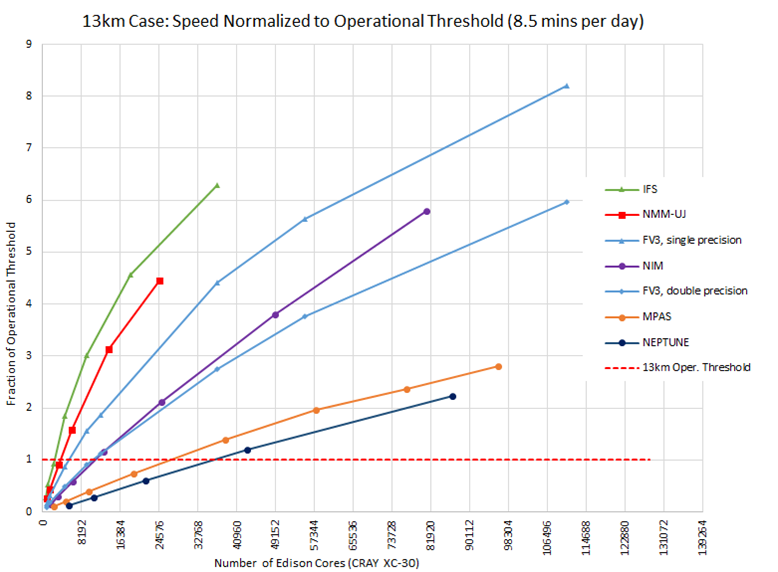
\includegraphics[width=.45\textwidth]{IFS_speed}	& 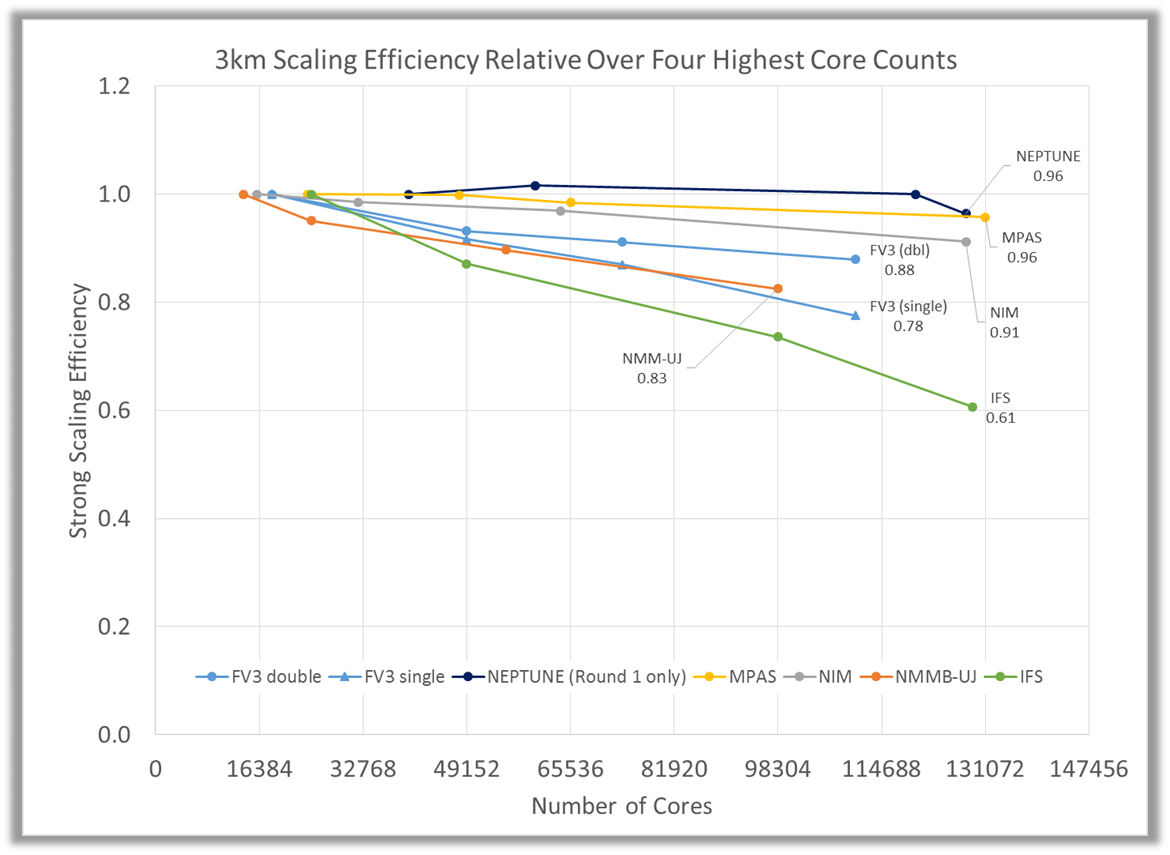
\includegraphics[width=.45\textwidth]{IFS_scaling}	\\
			\textbf{IFS speed}	&	\textbf{IFS scaling}
		\end{tabular}
	\end{center}
	%
\end{frame}
%
%%%%%%%%%%%%%%%%%%%%%%%%%%%%%%%%%%%%%%%%%%%%%%%%%%%%%%%%%%%%%%%%%%%%%%
%
\begin{frame}
	%
	\frametitle{The future?}
	%
	\begin{myitemize}{3ex}
		\item As machines get larger, there's a trend towards methods requiring less communications:
			%
			\begin{myitemize}{1ex}
				\item spectral $\rightarrow$ finite differences
				\item implicit (trapezium) $\rightarrow$ explicit (Runge-Kutta)
				\item Lagrangian $\rightarrow$ Eulerian
			\end{myitemize}
			%
		\item Maybe intermediate solutions such as HEVI (Horizontal Explicit, Vertical Implicit) are the future?
			%
		\item There's always a tradeoff between accuracy and computational cost
			%
		\item Power consumption may become a bigger challenge than communications
			%
	\end{myitemize}
	%
\end{frame}
%
%%%%%%%%%%%%%%%%%%%%%%%%%%%%%%%%%%%%%%%%%%%%%%%%%%%%%%%%%%%%%%%%%%%%%%
%
\end{document}
